\chapter{Lab 5 Results --- Training Pipeline Diagnostics}
\label{app:lab5}

Lab~5 uses \textbf{controlled ablation}: the same tiny GPT model (4 layers, 128 hidden, $\sim$830K params) is trained on Tiny Shakespeare under different pipeline configurations. The central thesis: training logs can lie---a correct architecture with a broken pipeline produces numbers that look reasonable but mean the wrong thing.


\section{Exp 0: Tokenizer and Vocabulary Size Sweep}

\textbf{Question:} Can we compare raw cross-entropy loss across tokenizers?

\textbf{Setup:} Same corpus (Tiny Shakespeare, 1.1\,MB), same model architecture, same 1500 training steps. Four tokenizers trained on the same corpus: character-level ($V{=}65$), BPE $V{=}256$, BPE $V{=}1000$, BPE $V{=}4000$.

\begin{center}
\begin{tabular}{lrrrr}
\toprule
Config & Vocab & Bytes/Token & Raw CE & Bits-per-Byte \\
\midrule
char     &    65 & 1.00 & \textbf{2.14} & 3.09 \\
BPE-256  &   256 & 1.96 & 3.62 & 2.66 \\
BPE-1000 &  1000 & 2.79 & 4.32 & 2.23 \\
BPE-4000 &  4000 & 3.70 & 5.45 & \textbf{2.12} \\
\bottomrule
\end{tabular}
\end{center}

\textbf{Key finding:} Raw CE loss and bits-per-byte rank in \emph{opposite order}. A student looking only at raw loss would conclude char-level (2.14) is best; normalized to bits-per-byte, BPE-4000 (2.12) is actually best. Raw per-token loss is not comparable across tokenizers because tokens carry different amounts of information.

\begin{figure}[ht]
\centering
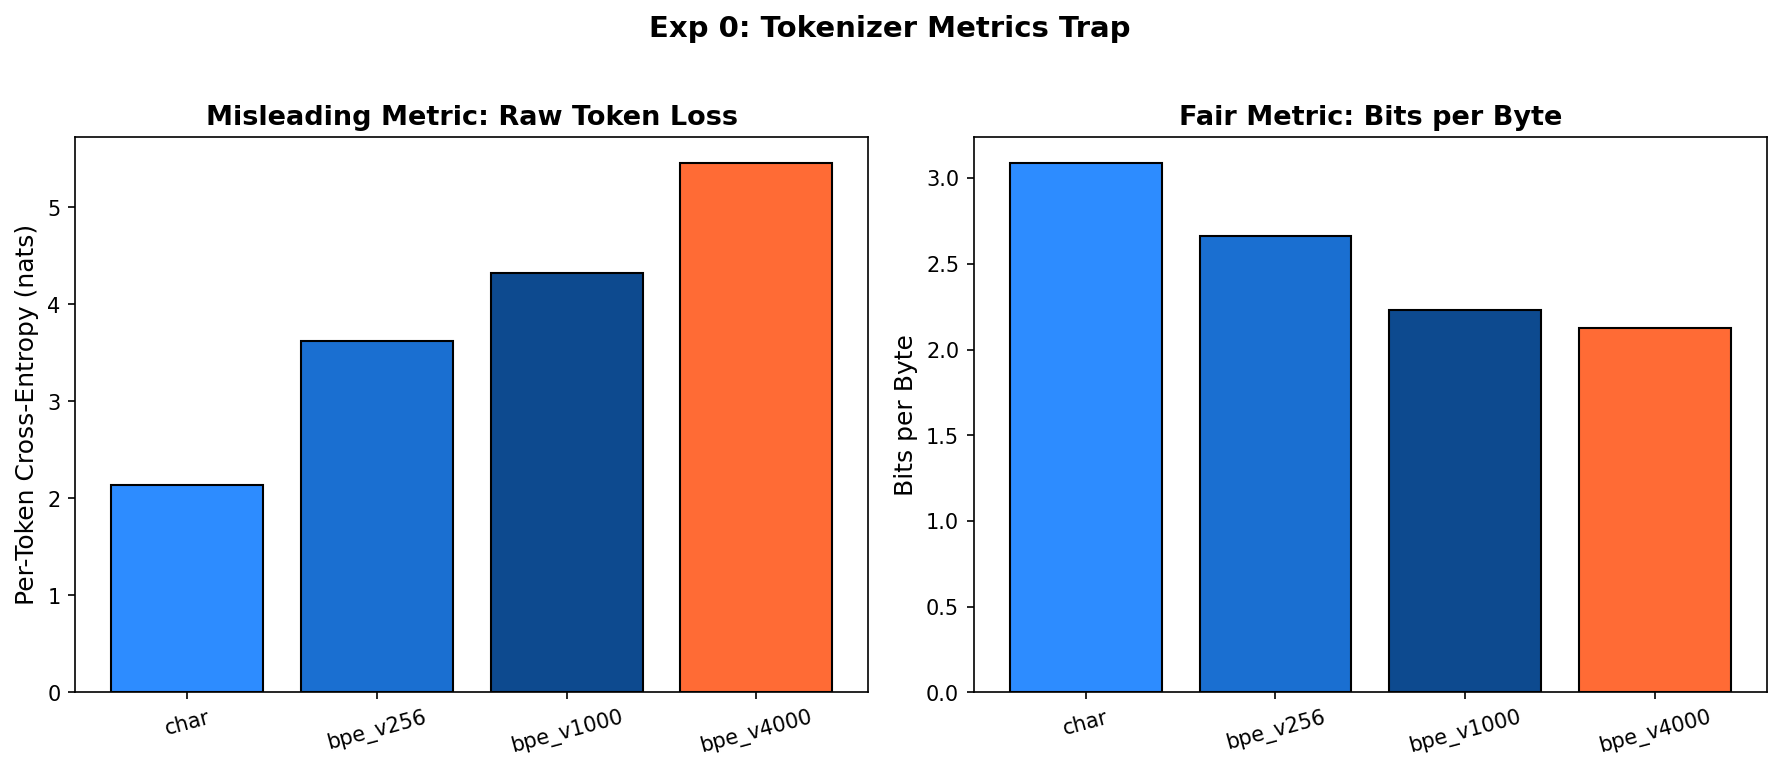
\includegraphics[width=0.9\textwidth]{labs/ch05/answers/figures/exp0_tokenizer_sweep.png}
\caption{Left: raw CE loss appears lowest for char-level. Right: bits-per-byte reveals that BPE-4000 actually achieves the best compression. The two metrics rank the tokenizers in opposite order.}
\label{fig:lab5_exp0_sweep}
\end{figure}

\begin{figure}[ht]
\centering
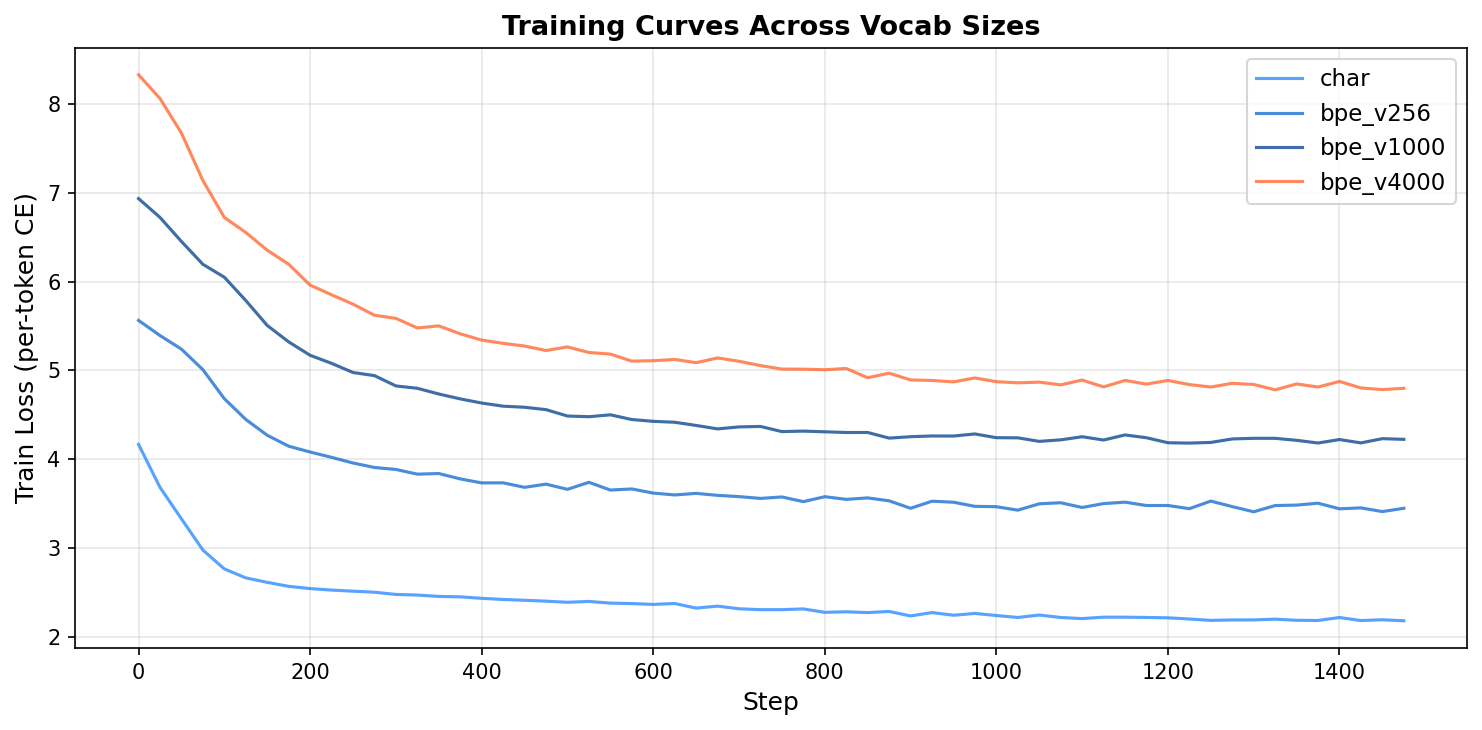
\includegraphics[width=0.9\textwidth]{labs/ch05/answers/figures/exp0_training_curves.png}
\caption{Training curves (raw CE) for all four tokenizers. Char-level converges to the lowest raw loss, but this is misleading---each token predicts only one character.}
\label{fig:lab5_exp0_curves}
\end{figure}


\section{Exp 1: Learning-Rate Schedule Ablation (Centerpiece)}

\textbf{Question:} If loss is decreasing, does that mean the schedule is good enough?

\textbf{Setup:} Same model, same char-level tokenizer, 2000 steps. Three schedules:
\begin{enumerate}
\item \texttt{too\_high}: $\eta{=}0.1$, no warmup, no gradient clipping
\item \texttt{no\_warmup}: $\eta{=}10^{-3}$, constant, with clipping
\item \texttt{warmup\_cosine}: $\eta{=}10^{-3}$, 200-step warmup + cosine decay
\end{enumerate}

\begin{center}
\begin{tabular}{lrl}
\toprule
Schedule & Final Val Loss & Observation \\
\midrule
too\_high       & 3.34 & Loss drops but plateaus high; text is random chars \\
no\_warmup      & 1.58 & Learns well; constant LR works for short training \\
warmup\_cosine  & 1.65 & Learns similarly; cosine decays too early in 2000 steps \\
\bottomrule
\end{tabular}
\end{center}

\textbf{Key finding 1:} LR $100\times$ too high does not produce NaN---it silently converges to a trivial solution (predicting common characters without learning structure). Generated text is gibberish despite a ``reasonable-looking'' loss of 3.3.

\textbf{Key finding 2:} For tiny models with short training budgets, warmup+cosine $\approx$ constant LR. The cosine advantage emerges at longer horizons where the late-stage low-LR refinement matters.

\begin{figure}[ht]
\centering
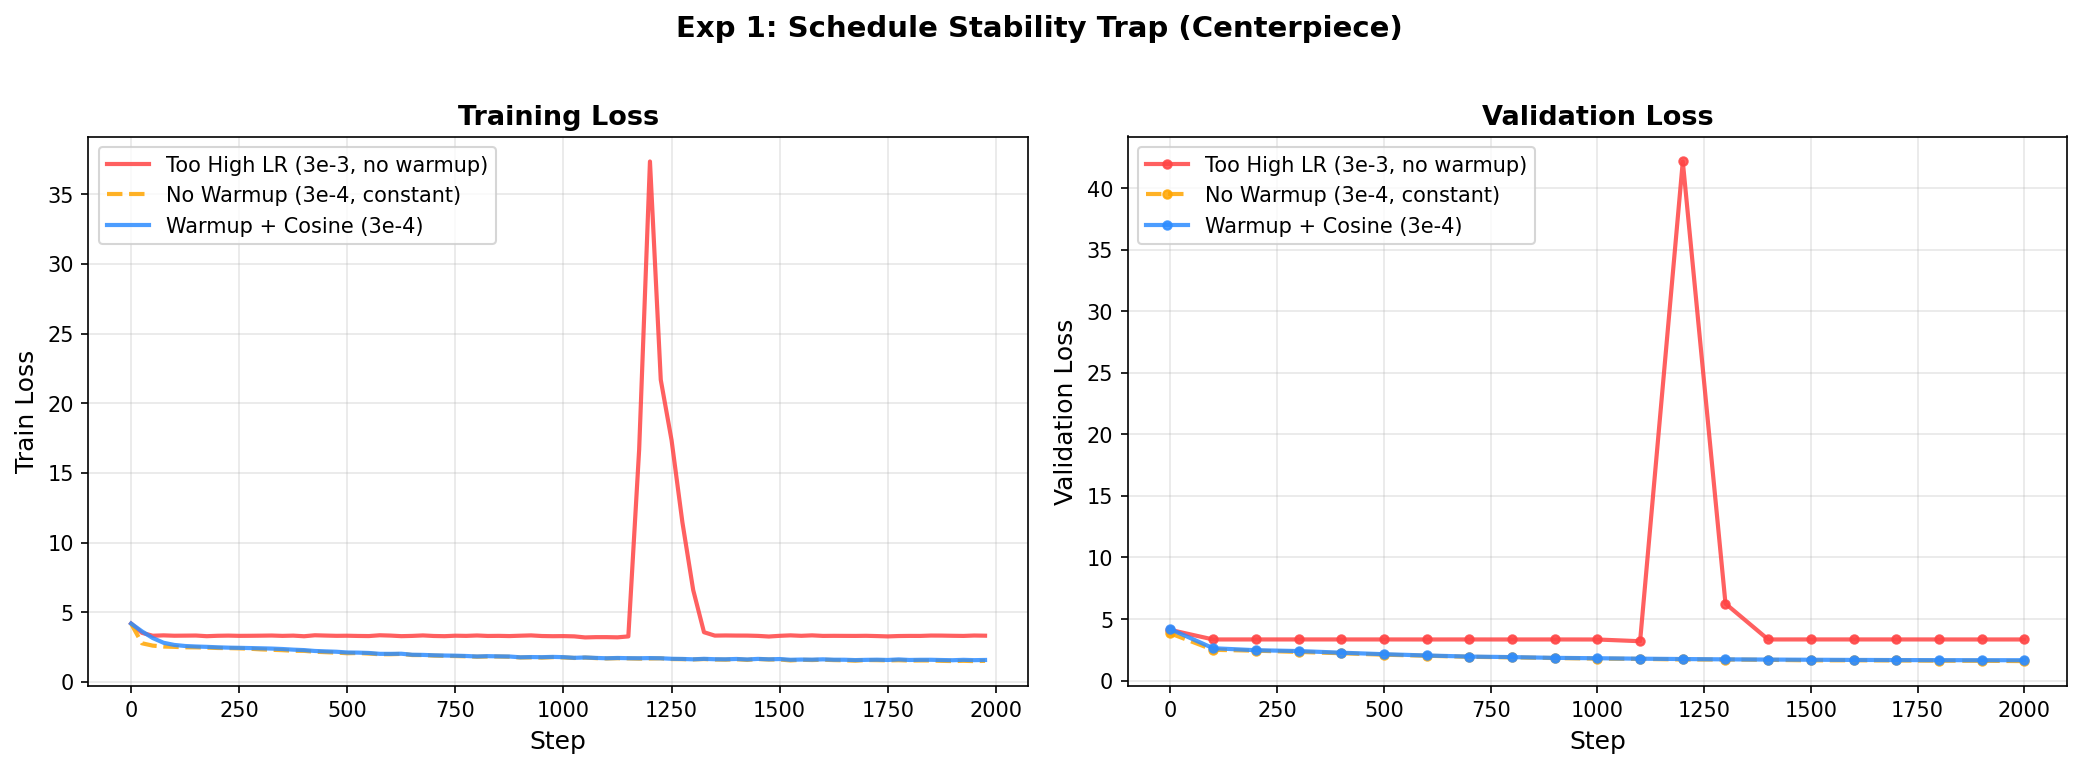
\includegraphics[width=0.9\textwidth]{labs/ch05/answers/figures/exp1_lr_schedule.png}
\caption{Three LR schedules produce dramatically different outcomes. The \texttt{too\_high} run's loss decreases but the model learns nothing useful---a silent failure.}
\label{fig:lab5_exp1}
\end{figure}


\section{Exp 2: Checkpoint Resume Ablation}

\textbf{Question:} Is saving model weights sufficient for resuming training?

\textbf{Setup:} Train to step 1000 (Phase~1, warmup+cosine over 1000 steps), then resume to step 2000 with different checkpoint contents:
\begin{itemize}
\item \texttt{uninterrupted}: full 2000 steps, no interruption (reference)
\item \texttt{full\_resume}: restore model + optimizer + scheduler + step
\item \texttt{model\_only}: restore only model weights
\item \texttt{no\_scheduler}: restore model + optimizer, restart scheduler from scratch
\end{itemize}

\begin{center}
\begin{tabular}{lrr}
\toprule
Run & Final Val Loss & Gap vs Reference \\
\midrule
uninterrupted  & 2.029 & --- \\
full\_resume   & 2.181 & +0.152 \\
model\_only    & 2.207 & +0.178 \\
no\_scheduler  & \textbf{1.914} & \textbf{$-$0.115} \\
\bottomrule
\end{tabular}
\end{center}

\textbf{Key finding 1:} \texttt{model\_only} resume performs worst---the optimizer must re-estimate momentum and variance from scratch, wasting early resume steps.

\textbf{Key finding 2:} \texttt{no\_scheduler} \emph{accidentally beats the reference}. Resetting the scheduler gives the model a second warmup with fresh high LR in Phase~2. This unplanned LR restart provides extra training signal---\textbf{a bug that looks like an improvement}. In production, such accidental restarts would waste the fine-grained convergence from Phase~1.

\textbf{Lesson:} A checkpoint is not just weights. It is the full training state. And metrics can improve for wrong reasons---always verify whether an ``improvement'' is robust.

\begin{figure}[ht]
\centering
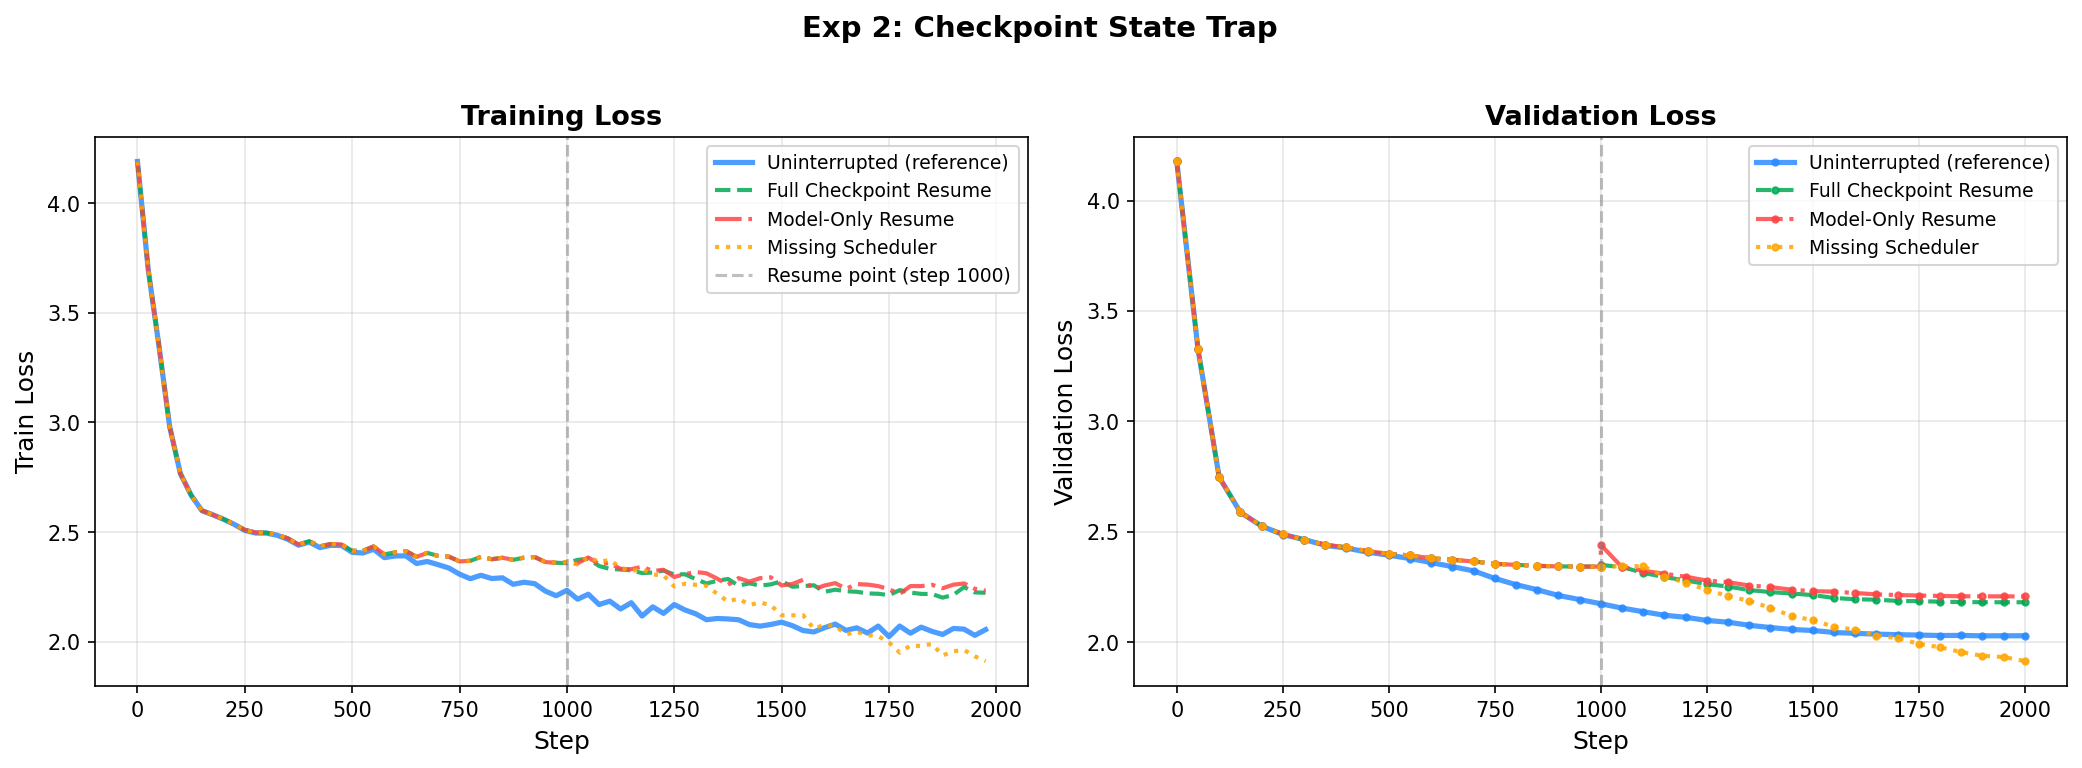
\includegraphics[width=0.9\textwidth]{labs/ch05/answers/figures/exp2_checkpoint_resume.png}
\caption{Four resume strategies produce different Phase~2 trajectories. The \texttt{no\_scheduler} run achieves the lowest final loss---but for the wrong reason (accidental LR restart).}
\label{fig:lab5_exp2}
\end{figure}
